\documentclass[11pt]{article}

\usepackage[utf8]{inputenc}
\usepackage[T1]{fontenc}
\usepackage[head=26pt, a4paper, margin=1.2in, top=1.4in, bottom=1.75in]{geometry}
\usepackage{fancyhdr}
\usepackage{lastpage}
\usepackage[hidelinks, colorlinks, urlcolor=blue, linkcolor=black,citecolor=magenta]
{hyperref}
\usepackage{amsmath}
\usepackage{amsthm}
\usepackage{amssymb}
\usepackage{graphicx}
\usepackage{float}
\usepackage{listings}
\usepackage{mathtools}
\usepackage{enumitem}


\usepackage{indentfirst}
\usepackage{a4wide}
\usepackage{color}
\usepackage{lipsum}
\usepackage{multicol}
\usepackage{tikz}
\usetikzlibrary{arrows,shapes,positioning}

% ---------------- Page and margin/header/footer Setup -----------------
\pagestyle{fancy}
%\fancyhf{} % Clears header and footer
\fancyhead{}
\fancyfoot{}
\lhead{ACS --- Assignment 3}
\rhead{DIKU}
\lfoot{Page \thepage\ of \pageref{LastPage}}
\rfoot{Nicolai Jørgensen \\ Yiran Zhang}
\renewcommand{\headrulewidth}{0.4pt}
\renewcommand{\footrulewidth}{0.4pt}
% ----------------------------------------------------------------------

\newtheorem{mythm}{Theorem}
\newtheorem{mydef}{Definition}

\DeclarePairedDelimiter{\ceil}{\lceil}{\rceil}
\newcommand\numberthis{\addtocounter{equation}{1}\tag{\theequation}}

\newcommand{\HRule}{\rule{\linewidth}{0.5mm}}

\title          {Assignment 3}
\author         {Nicolai Jørgensen and Yiran Zhang}

\begin{document}

\maketitle
\newpage

\section{Recovery Concepts}
\begin{enumerate}
	\item
    In a system implementing force and no-steal it is not necessary to implement
    a scheme for redo, because all committed transaction have been
    written to disk at the time of a crash. It is also not
    necessary for undo, since all dirty writes have not been written to disk at
    the time of a crash.
	\item
    Non-volatile storage retains data even when power goes off, while the
    information in stable storage is (theoretically) completely permanent.
    
    By this we mean that events might result in a loss of data on stable
    storage, but the probability of data loss is negligible. The non-volatile
    storage is much faster than stable storage in terms of access time.
    
    So non-volatile storage survives system crashes, but it is still subject to
    media failure. In our model, we assume stable storage to not experience
    media failures.
	\item
    The log tail needs to be forced to disk in two cases: When a transaction is
    committed or when pages are written to disk.

    For the first case, if a transaction made a change and committed, the
    no-force approach means that some of the changes may not have been written
    to disk at the time of subsequent crash. Without a record of these changes,
    there would be no way to ensure that the changes of a committed transaction
    survive crash.

    For the second case, if the dirty write is written to the disk in yet
    uncommitted transaction at the time of subsequent crash, Without a record
    of these changes, there would be no way to undo the changes.

    These rules are sufficient for durability because they support undoing
    modifications and ensure all actions of committed transactions survive
    system crashes and media failures.
\end{enumerate}

\section{Discussion on the Performance Metric}
  \begin{enumerate}
    \item
      When generating books for our experiment we vary the following parameters:
      Author, title and ISBN. The author and titles are random strings of alphabetic
      characters with fixed length and the ISBNs are numerically increasing from 1.
      Depending on the data structure that keeps the books, the fact that ISBNs are
      not distributed realistically might impact performance, but most implementations
      will use some form of map or hashing that will make this irrelevant. Still, it
      should be kept in mind that this might negatively impact the predictions of our
      metrics. Another reasonable strategy for ISBN generation is simply to pick a
      uniformly random positive integer. Even better, a large amount of real ISBNs
      could be used as a source.

      Our experiments were run on a single machine with an Intel Core i5-3337U
      processer. It has 2 cores each capable of running 4 threads. The processor has
      3MB of cache shared between threads. The machine has 8GB of RAM and runs 64-bit
      Windows 10.

      We do our measuring for varying number of concurrent clients accessing the
      bookstore. We don't do multiple experiments for the same number of
      clients, so we can't apply any statistical methods to it.

    \item
      Here is the graphs for our experiments:

      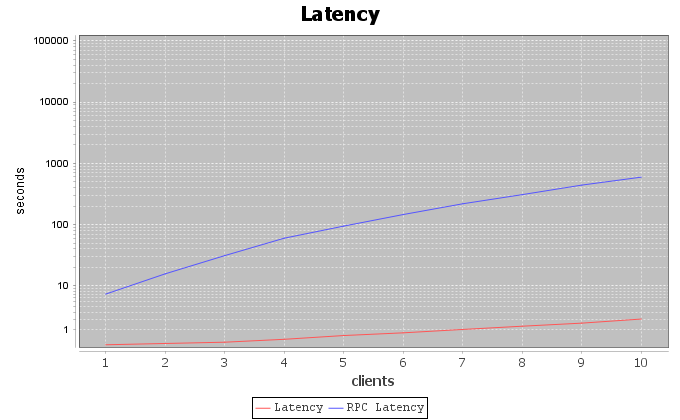
\includegraphics[scale=0.5]{latency}

      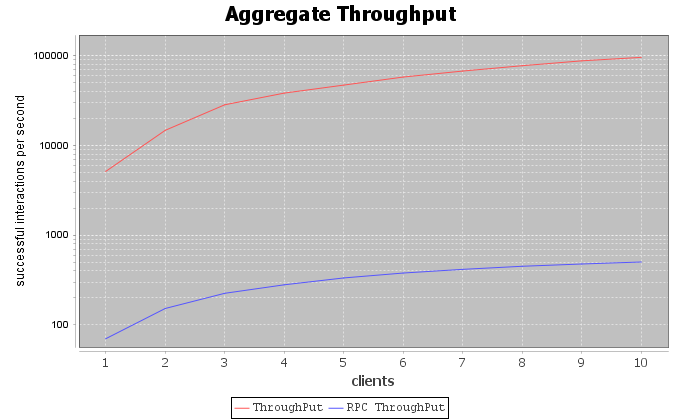
\includegraphics[scale=0.5]{throughput}

      The first obvious trend to notice is that the local computations are
      faster than the remote ones by orders of magnitude. This matches our
      expectations, since RPCs have the entire overhead of transferring the data
      through HTTP.\\

      Another thing to notice is that throughput increases as we add concurrent
      clients. We are testing against the basic bookstore implementation with no
      concurrency control at all, so every thread can access any data at all
      times. That throughput increases is then expected because we take
      advantage of the multiple processor threads.

      In the case of RPC throughput, we expect that the throughput gain comes
      from the serialization and sending of data being parallelized, since the
      actual bookstore operations happen on the single-threaded server. In this
      case though, the serverside computations are all relatively cheap, so they
      do not dominate performance.\\

      When clients increase, so does the latency for each client, especially in
      the case of RPCs. In the case of local computation access to resources get
      more frequent and should impact performance. In the case of RPC latency,
      the server needs to respond to all requests, which also impacts
      performance.

    \item
      In order to evaluate how well our metrics should predict the actual performance
      of the system, we need to look at how our metrics have been chosen. In this
      case, by the distribution of tasks, we have strived to simulate what we believe
      to be an average workload. We deliberately generate buy orders of less than 10
      books and similarly add small sets of books.

      Obviously, we don't actually \textit{know} that the workload is
      realistic., In a real life scenario, we would probably use some form of
      logging during normal operation and using the log to inform our workload
      generation. For this case though, we believe the strategy is good. It
      should produce metrics close to the actual service performance.\\

      However, the strategy does not test for abnormal workloads at all. For example,
      a big release could prompt a large spike in users trying to buy the exact same
      book, or a number of clients could put in huge buy orders of many different
      books which might similarly stress the system.

      In order to effectively test for these cases, some amonut of foresight must be
      involved. For example, if we anticipate a big release, we should test the
      service against the abnormal workload that we expect will occur.
  \end{enumerate}

\end{document}
